\section{系统测试与结果分析}

\subsection{测试目标与测试环境}

系统测试重点围绕以下问题展开：
\begin{enumerate}[leftmargin=2em]
  \item 中间表示是否能稳定校验；
  \item 分析、生成、合并流程是否可正常运行；
  \item CLI 与 Web UI 是否能够正确调用核心能力；
  \item 对典型样例，系统是否能给出完整输出；
  \item 异常输入是否会被合理拦截。
\end{enumerate}

测试环境基于项目自带 Python 虚拟环境执行，核心验证命令包括自动化测试与样例构建命令。由于当前仓库尚未接入 Onshape 在线编译回读闭环，因此本文测试重点放在本地逻辑正确性、脚本生成完整性和接口调用一致性上。

\subsection{自动化测试结果}

在项目当前版本下，执行自动化测试命令后，共有 50 项测试全部通过，执行时间约为 2.37 秒。进一步统计覆盖率后，项目总代码覆盖率达到 82\%。主要覆盖对象包括 \texttt{models}、\texttt{analysis}、\texttt{generation}、\texttt{application}、\texttt{cli}、\texttt{io} 和 \texttt{webui} 等模块。

\begin{table}[H]
  \centering
  \caption{系统核心验证指标}
  \label{tab:main-metrics}
  \begin{tabular}{p{5.2cm}cc}
    \toprule
    指标 & 数值 & 说明 \\
    \midrule
    自动化测试通过数 & 50 & 本地 \texttt{pytest} 结果 \\
    代码覆盖率 & 82\% & \texttt{pytest --cov} 统计结果 \\
    支持零件形状数 & 5 & 受限任务域设置 \\
    冷拉延模具样例成功率 & 5/5 & 全部零件成功生成 \\
    \bottomrule
  \end{tabular}
\end{table}

覆盖率明细显示，覆盖相对较低的部分主要是 \texttt{webui/server.py} 的 HTTP 处理细节与部分兼容层入口文件。这说明系统已经对核心业务逻辑做了较充分验证，但在端到端浏览器交互方面仍有继续补充测试的空间。

\begin{figure}[H]
  \centering
  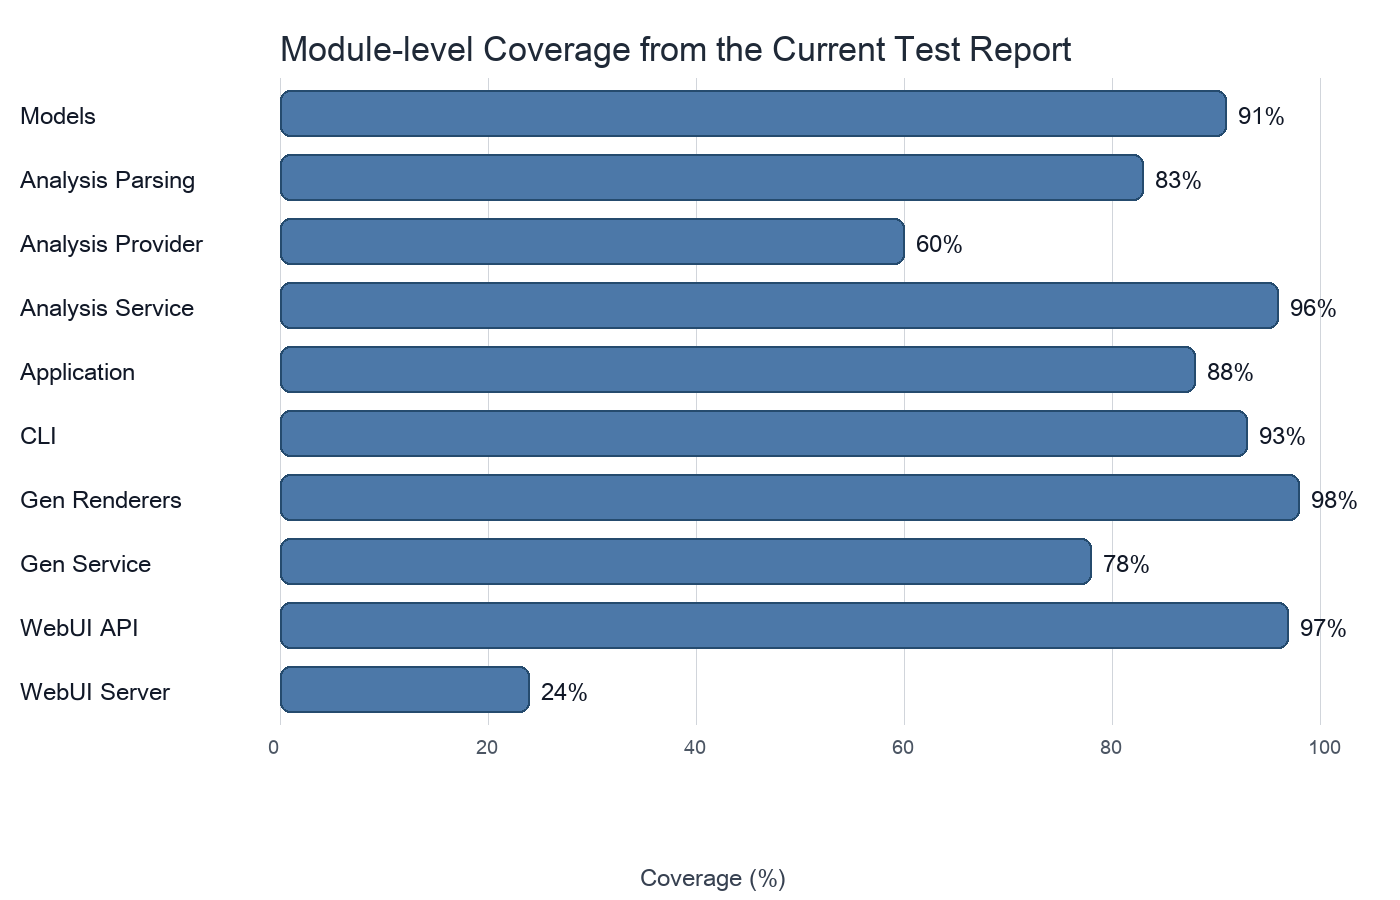
\includegraphics[width=0.94\linewidth]{figures/coverage_chart_python.png}
  \caption{基于真实覆盖率报告绘制的模块级覆盖率对比图。该图由 Python 脚本自动生成，并作为评测结果图直接纳入正文。}
  \label{fig:coverage-chart}
\end{figure}

\subsection{典型样例验证}

为了验证系统完整链路，本文选取仓库内置的“冷拉延模具”需求文本作为典型样例进行构建测试。该样例描述了上模座、下模座、凹模、压边圈和凸模五个主件，并给出了关键尺寸约束。执行构建命令后，系统成功输出一个结构化 Plan 文件、一个完整 FeatureScript 文件，并实现 5/5 零件全部生成成功。

从生成结果可见，系统将自然语言需求转换为一个包含 5 个零件和 4 条装配关系的装配 Plan。其中，下模座和上模座被识别为 \texttt{box}，凸模被识别为 \texttt{cylinder}，凹模和压边圈被识别为 \texttt{hollow\_cylinder}。在 FeatureScript 输出中，系统进一步将这些零件映射为立方体、圆柱体和布尔减运算等稳定几何操作。

该样例验证说明，在受限任务域内，系统不仅能理解结构性需求，还能形成符合模板约束的参数化输出。

\subsection{结果分析}

从测试与样例结果看，本文系统具有以下优点：一是结构清晰且工程闭环完整；二是中间表示设计有效，能够通过 Plan 约束收缩自然语言带来的不确定性；三是演示友好，CLI 与 Web UI 复用同一套服务逻辑；四是错误处理较为明确，需求缺失、Plan 非法或零件生成失败时都能给出可理解反馈。

但系统也存在明显局限：
\begin{enumerate}[leftmargin=2em]
  \item 目前仅支持五种基础零件形状，无法覆盖更复杂的孔、圆角、倒角和复杂装配约束；
  \item 尚未与 Onshape 编译结果建立自动闭环，因而当前验证重点仍是“脚本生成正确性”，而非“云端 CAD 执行正确性”；
  \item 当前缺少真实用户实验和大规模需求集合测试，无法从统计意义上评价系统在开放域需求下的鲁棒性；
  \item 分析阶段仍依赖外部大模型接口，在没有 API Key 的一般场景下无法完成通用需求分析，当前 fallback 仅服务于内置演示样例。
\end{enumerate}
